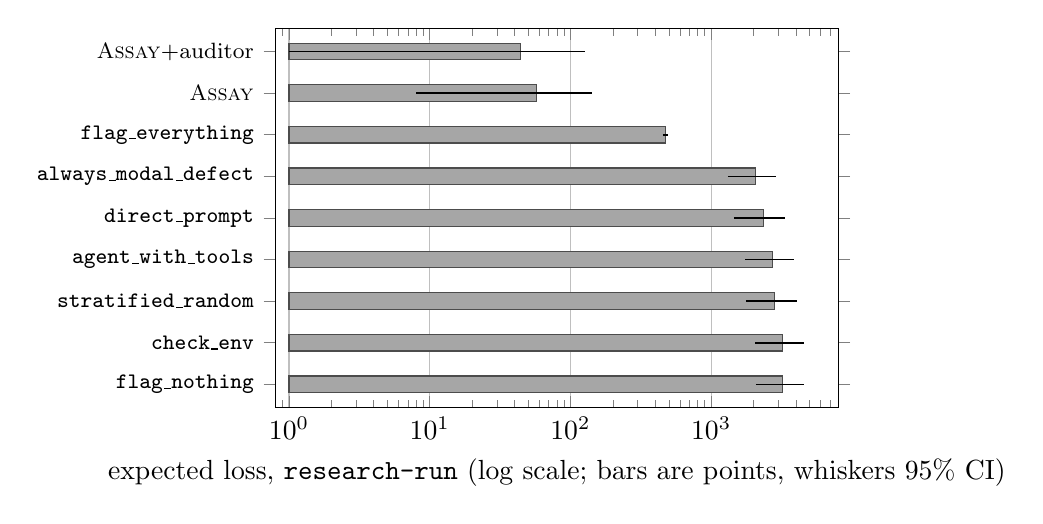
\begin{tikzpicture}
\begin{axis}[xbar, xmode=log, width=0.72\linewidth, height=6.4cm, xmin=0.8, xmax=8000,
  symbolic y coords={flagnothing,checkenv,stratifiedrandom,agentwithtools,directprompt,alwaysmodaldefect,flageverything,assay,assayplusauditor}, ytick=data, yticklabels={{\texttt{flag\_nothing}},{\texttt{check\_env}},{\texttt{stratified\_random}},{\texttt{agent\_with\_tools}},{\texttt{direct\_prompt}},{\texttt{always\_modal\_defect}},{\texttt{flag\_everything}},{\textsc{Assay}},{\textsc{Assay}+auditor}}, yticklabel style={font=\footnotesize},
  xlabel={expected loss, \texttt{research-run} (log scale; bars are points, whiskers 95\% CI)},
  bar width=6pt, xmajorgrids, enlarge y limits=0.07]
\addplot[fill=black!35, draw=black!70] coordinates {(3232.0,flagnothing) (3216.0,checkenv) (2838.0,stratifiedrandom) (2746.0,agentwithtools) (2343.0,directprompt) (2055.0,alwaysmodaldefect) (474.0,flageverything) (57.0,assay) (44.0,assayplusauditor)};
\draw[black, line width=0.6pt] (axis cs:2080.0,flagnothing) -- (axis cs:4560.0,flagnothing);
\draw[black, line width=0.6pt] (axis cs:2056.0,checkenv) -- (axis cs:4552.0,checkenv);
\draw[black, line width=0.6pt] (axis cs:1767.0,stratifiedrandom) -- (axis cs:4071.0,stratifiedrandom);
\draw[black, line width=0.6pt] (axis cs:1753.0,agentwithtools) -- (axis cs:3883.0,agentwithtools);
\draw[black, line width=0.6pt] (axis cs:1451.0,directprompt) -- (axis cs:3366.0,directprompt);
\draw[black, line width=0.6pt] (axis cs:1315.0,alwaysmodaldefect) -- (axis cs:2909.0,alwaysmodaldefect);
\draw[black, line width=0.6pt] (axis cs:453.0,flageverything) -- (axis cs:492.0,flageverything);
\draw[black, line width=0.6pt] (axis cs:8.0,assay) -- (axis cs:142.0,assay);
\draw[black, line width=0.6pt] (axis cs:1.0,assayplusauditor) -- (axis cs:126.0,assayplusauditor);
\end{axis}
\end{tikzpicture}
